\documentclass[preprint,nocopyrightspace]{sigplanconf}
%twocolumn
\usepackage{epsfig}
%\bibliographystyle{abbrvnat}

\begin{document}

\title{
PLT Scheme Scene Graph: An Application of Mixin for Construction of Graphics
Scene Data Structure.}

\authorinfo{Seungkeol Choe\and Matthew Flatt}
           {School of Computing, University of Utah\\
%             50 S. Central Campus Dr. 3190, Salt Lake City, UT 84112\\
             \texttt{\{skchoe, mflatt\}@cs.utah.edu}}

\maketitle

\begin{abstract}
This paper presents a high level API for constructing scene graph structure in
PLT Scheme. That is built upon the SGL, the OpenGL binding in scheme and
supplies the basic primitive three dimensional objects. We add basic graphics
operations for visualization and interactive manipulation of the objects in
the scene or the whole viewing operations. The focus of this paper is to show
the structure of communications between a domain-specific structure and
visualization structure. We bring what the Mixin class features and apply it
to the way of constructing a structure for visualization. The transformation
from the core domain structure to visualizatoin structure is to applying a few
procedures for converting the two structures and domain structures to Mixin
class. This approach helps the client software developer focus on the domain
data construction, management and conversion which is free of constructing
visualization structure. 
\end{abstract}

\section{Introduction}
\label{intro}
 Scene graph\cite{Scenegraph} has been a wide spread structure for
 constructing three dimensional objects and maanaging the collection of objects in computer
 graphics. Since introduced in 1990s, it has been keeping evolved and improved
 by many different commercial or open source programming packages. Especially,
 in developing a realtime interactive graphics software library, some take the
 the approach with OpenGL\cite{OpenGL} as a backend module
 and support high-level programming interface for simple, and intuitive tool for graphics programmers.

 When it comes to software development in actual application fields, the
 design and implementation of structure for representing a visualization
plays a role as not only for visualzation of object and result of domain specific operations but also
 support for input operations that is to say, interface to take user's
 interaction. Also it also gives visualization of user's input itself to give
 better interaction to user such as widget helper in three dimensional
 space. In this sense, the domain data structure and communication with scene structure is very important in system design to give application programmer a better understanding to work with. 

For example, in most of graphic software for modeling, animation, etc, there exist a software specific structure to manage the data to receive user command and visualize the resultsuch as CSG operation or generation of new position information from motion capture device. in geographic information system (GIS), the software is designed to maintain a core data structure which interfaces to GIS database engine, GPS data receiver, or information visualization module. At last, chemistry simulation software, most of atom, molecule, protain data structure exists which is separated from visualzation structure to support multiple interaction reading or writing the data efficiently.

As shown in detail by examples, we focus on the design of two structures and their relations each other: core system structure which is designed by the domain specific data properties, and a visuazliation structure which mainly contains how to draw and manage the graphics object and how to receive and responds the interaction from the software users. The main concern is to choose an efficient design for the data comunication and intuitive programmability between the structures.
 
We present a simple prototype system to deal with the issue. By showing the
application of Mixin interface class as a container of specification and
implementation of the commnunication to build interafce between the two: core
and visualzaiton structures. Once we have the interface class desinged by the
original requirement of the software specific to a domain, the programmers is
more able to focus on how to build the logic for each actaul object and
operation on it. 

In the software development aspect, this implementation can be interpreted into model, view, and conller sub parts. We mostly focus on the inter-relation between model and view parts and we implement controller part using PLT Scheme helper interfaces.
\begin{itemize}
\item The Controller part rely on the structure and interface function in MrEd. What the functions do is to get help for supporting event generation and the callback functions containing the idea of how to change the objects and environment in view strucure. This is more described in \ref{STR_VIZ}.
\item The main charateristic of this paper is to help software designer in given specific
domain to more focus on managing domain data structure because most of
applicaion need operations of creating, applying business logic to the data,and 
managing it. Visualziation is located in a part of final result presentation
or a tool for determining the input values in interactive software environment. \ref{CM_SG} deals with the generation of scene graph in view module from model parts.
\item The view part of the structure is totally managed in high level by this implementation. Though
the amount of support in the kinds of 3 dimensional objects is minimal, this will show the example that how to design a whole system structure model in terms of the three sub structures. \ref{STR_VIZ} and \ref{STR_SLN} describe the 3 dimensional rendering and object selection.
\end{itemize}

This paper comes with the following structure. In background section, we reviewed all components used to build the prototype and how the idea is used, and how it is beneficial in actual case in general high level. In implementation section,  we showed the key functions working for specific example situations. We close this paper with with some evalaution about the approach and future direction of development.

\section{Related Works}

As introduced in Chapter \ref{intro}, scene graph has been a useful tool for three dimensional graphics visualization. In this section we overview representative examples of application programming interface.
\begin{itemize}
\item Open Inventor \cite{OpenInventor}\\
Open Inventor is the first implementation of the main idea of three dimensional scene representation. Not only presenting the complex graphics object, it showed the elements of graphics scene composition environment by object oriented programming model. These include the class for camera,lights, mouse or trackball and various graphical manipulator widgets for interactive handler. It persues multi-platform execution environment, its own data file format and printing functionality. Currently, its source code becomes open source so that various graphics programmers can update the feature for their own purposes.
\item Java 3D \cite{Java3D}\\
As an official three dimentional application programming interface, it is introduced following its 2 dimensional part in Java software package. Its programming model is following object oriented frame work as well. But its class hierarchy implementation for scene description has been more structurized than Open Inventor. For example, the concepts such as Virtual Universe, Locales, and Branches shows more details by the role of each components of object in a scene. 

Since it is built on top of Java technology, its feature including platform dependency also valid and it has also been suffered from the performance issue because of the nature of deta intensivity of three dimensional graphics programming. JoGL\cite{jogl} OpenGL bindings for java has been popular alternative for Java3D because of it maintains the feature of Java and because it is a low level API, it showes a competitive performance which is useful replacement of high level API's 
\item Open Scene Graph \cite{OpenSceneGraph}\\
This API is a product of a project originated from open source porting of IRIS performer high level navigation and visualization API. As its starting purpose represents, its main goal has been on visualization of huge amount of data sets which becomes nowadays a main stream target of graphics APIs. So from the begining, it has more focused for data optimization such as various culling techniques: view-frustum, occultion, abstraction in component design considering level of detail, scene object sorting. 

Not only for the class design, it started with geometric models that can process sets of attributs for object. As getting expended in open source community, it equipped the utility for interfacing various object file formats, image file supports. Also the idea for node implementation of visual simulation, interactive manipulation, shadow and anti-aliasing has been presented. It is currently the representative implementation for scalable computing environments; multi-processing of node on mult-cpu, gpu, and distributed computing environements. 
\end{itemize}

The object oriented implementation is a common part of the above example implementations. PLT Scheme Scene Graph takes an approach to show simplified relalization of scene graph concepts to give a quick and easy access to visualize three dimensional object in the scene. So the support of high level modeling and handling of graphics objects is more focused than supporting high level functionality such as scene management for fast visualization, control of level of details. Implemented in PLT Scheme, the abstraction of modeling object and composition of global scene structure is functional. So the apply the change of object node, updating an attribute of a part of node is made by constructing corresponding node and building new scene graph node structure. This feature is very useful to maintain scene graph because the management is usally envoked by the state change in domain specific data model and structure. So the unified transformation between constrution and modification from domain structure to scene graph allow the software developper to concentrate more on data model aspect which interfaces various of source of data input modules.

\section{Background Concepts and Structure of PLT Scheme Scene Graph}
\subsection{Scene graph and graphics components}
Scene graph is a simply acyclic tree structure whose nodes are defined by graphics object, rendering attributes, object for receiving and responding events. It accepts external nodes in its connection in general to allow extension. The design indetail is up to all different implementation by the complexity of its target system. Currently, the developemnt of scene graph moves towards for allowing the structure to handle a huge number of nodes efficiently such as objec culling, space partitioning and to add new graphics and computing technology like raytracing and distributed node processing.\cite{OpenSceneGraph}. 

In this prototype, we design the scene graph as simple as possible so that in the future it's easy to add new feature and more focus on the structure itself, not the node in detail. It has only two kinds of nodes: scene-node and scene-leaf-node which scene-node is a super structure of scene-leaf-node and scene-leaf-node is an only leaf node of the tree containing graphics primitive object information. When the same attributes in super and child appear at the same time, the one in child node overrides that of super by design. But the super node is used for defining sub-group information in the scene. Because, by definition, the sub-grouping can be applied in recursive fashion through out all tree structure, the tree designer has freedom how to create and manage the scene graph by the idea of original domain structure. The details of it will be dealt with in next section \ref{STR_VIZ}.

\subsection{SGL: OpenGL binding in PLTScheme}

The presented implementation is based on OpenGL binding(SGL)\cite{SGL} to PLT Scheme. The SGL is based on foreign function interface\cite{Barzilay04foreigninterface} of PLT Scheme, and defines scheme functions and predefined values with same name in OpenGL C-code. So it enables scheme programmer to directly work together OpenGL API. Also it defines a interfacing types which is called \texttt{ctype?} for formal variables of OpenGL API. So the type conversion and calling OpenGL API enables for OpenGL programming in PLT Scheme.

Currently, it supports procedures of OpenGL upto version 1.5 with some exception, there is no limitation for calling OpenGL library from constructing visualization components in our implementation. In addition, because SGL uses direct calling to OpenGL procedures, the way of coding is very close to normal C code except we need to define the original data type into SGL requires.From the fact that the supporting version limitation, it's enough to working with Microsoft OpenGL implementation 'opengl32.dll' to call function and building this prototype.

\subsection{Mixin}

Mixin\cite{Flatt06schemewith} is a form of class which is used to contain information about how to
express the class based on corresponding object and its operation. We use the concept when it needs to express parameterization of behavior from all different kinds of input. In this prototype, mixin works a key role for design the structure transformation between core and visualization structure. Mixin allows an infrastructure for the progammers to take care of structure coversion and object property conversion in separate fashion.

Mixin is useful when we design the infrastructure for the structure transformation. We can define the prototype of interfaces that is necessary for the conversion and a mixin class that check the implementation of the interfaces. At this stage the mixin is a single pack of information for the whole conversions. This is also possible because one of the property of mixin is that it is a the first class values. From these property, we define a parameterized structure for clearly defined interfaces and the client programmers have only to implement them.

\section{Implementation Details}
\subsection{Development goal}

The goal of this prototype implementation is three folds: One is to show how the interface between real software and visualization module should be designed for its simplicity, intuitivity, and future expansion, the second is to design inside structure of visuzalization part to be flexsible as a basis of future improvement, and the last is to see how Scheme functional programming language can handle the concept which has been mainly implemented by object oriented languages and how it can still bring the feature of the language itself.  In this aspect it is basically designed a simplified form of currently existing scene graph structure maintaining the structure and logic. As a result, the system tried to minimize the number of data states, incidents for reading and updating than that is in the traditional implementations.
  
\subsection{Definition of primitives}
The structure in which graphics primitives is defined and managed is designed by the operations around an object of renderer class and its subclasses. 
The operations here include primitive creation, calling render procedure, and responding to mouse events. 
There's the definition of super class render% of all renderer subclasses:
\begin{verbatim}
  (define r<%> (interface () render))
  (define renderer% (class* object% (r<%>)
      
      (init-field (xform ...))
      (init-field (material ...))
      (init-field (dl-id ...))
      (init-field (bbox ...))

      (public compute-bounding-box)
      (public render)
      (public pick)
      (super-new)).
\end{verbatim}
Here xform is a list of 4$\times$4 matrix for geometric transform of the primitive. 
The object of renderer class store an identifier, dl-id, for using it during the call of display list by re-paint event. 
The pick procedure is used to respond mouse event operation to help to figure out if the object itself is picked or selected. 
The class supply all necessary methods for them and it is instantiated during the transformation from domain structure to visualization structure. 
There are the interface functions that take appropriate adata, create the object, call the proper method of it when it is required. 
The primitives are defined hidden inside of the interfaces and used to create the renderer object. 
Appendix A[APPENDIX] lists all definition of primitives.

For scene rendering, we support the following graphics attributes to the primitives in the form of struct object:
\begin{verbatim}
(define-struct material (ambient diffuse specular 
                         shininess texture-object))
\end{verbatim} 
The first 3 elements are the structures of 4 float points and shiness is a single scalar value. The texture-object is defined by an image values and its dimension. The list of color values defines a texture image to be used in texture mapping to primitive object.

Each primitive contains its bounding box information in bbox which is created when the object is instantiated and used as a base dimension of object. The each node of scene graph has bounding box information calculated by that of renderer object.
 -
\subsection{The Construction and Management of Scene graph}
\label{CM_SG}
This section deals with the underlying framework about how the to construct the Scene graph using Mixin class in PLT Scheme. 
In the structure, Mixin class is a form of wrapping package for data conversion from domain structure to Scene graph structure. The creator of scene graph understand all data from domain structure as a form of Mixin. By the definition of mixin in terms of it's parameterizability by super class, the client programmer construct mixin super class. And the super class implements the interface in which we specified the required procedures.
The mixin class is defined by the child of the class and check if the super class gives proper implementation of the interface procedures. 
In this implementation, we simply require two procedures that help client be able to separate the conversion into two independent pieces.

\begin{verbatim}
(define convert-to-scene-graph<%>
  (interface ()
    object->renderer
    convert-to-scene-graph))

(define convert-to-scene-graph-mixin
  (lambda (%)
    (unless 
      (implementation? % convert-to-scene-graph<%>)
      (error "Need implemention: 
              convert-to-scene-graph interface\n"))
    (class* % ()
      (super-new))))

; in: mixin(child class), custom structure
; out: scene-graph
(define object-mixin->scene-graph
  (lambda (mxn stc)
    (let* ([mxn-obj (new mxn)])
      (send mxn-obj convert-to-scene-graph stc))))
\end{verbatim}

The code fragment above shows how the idea about Mixin is implemented. It has two group of procedures or classes. 
One is the procedures that take the implemented required interfaces and construct scene graph. 
The function ``object-mixin-$>$scene-graph'' takes the mixin class which could be understood how to transform domain structure to scene graph and domain structure itself as the first values. 
This property allows to parameterize the Mixin class as a data expression not the object as a data storage. 
The calls the method ``convert-to-scene-graph and returns generated scene graph structure. 

\begin{verbatim}
; parent class for mixin
(define flat-list->scene-root-node%
  (class* object% (convert-to-scene-graph<%>)
    (super-new)
    
    (define/public object->renderer 
      (lambda (points normals 
               texture-coords faces part-mtl-param)
        (obj-part->renderer points normals 
               texture-coords faces part-mtl-param)))
    
    (define/public convert-to-scene-graph 
      (lambda (flat-list)
        (flat-list->scene-root-node flat-list)))))
   

; child mixin class
; input: structure of flat-list
; use global(in this module) for conversion: 
;                flat-list->scene-root-node%
(define generate-scene-graph-from-flat
  (lambda (stc)
    (object-mixin->scene-graph 
      (convert-to-scene-graph-mixin 
        flat-list->scene-root-node%)
       stc)))
\end{verbatim}

The above code shows an example domain structure and how to call the infrastructure for transforming to scene graph. 
The term ``flat'' is an example structure which is a collection of groups whose elements are object constructed by various fish graphics object from importing ``obj'' file format. So the ``stc'' refers to the collection and ``generate-scene-graph-from-flat takes it and construct scene graph using pre-existing Mixin super class. As explained the Mixin class contains how to handle structure and element of domain structure to scene graph node and renderer structure. 

The next is the definition of {\tt flat-list->scene-root-node} which calls recursive function {\tt initialize-scene-node} 
\begin{verbatim}
  ;; fish-list -> root-node
  (define flat-list->scene-root-node
    (lambda (fl) ; (pair of fish-group)
      (when (not (empty? fl))
        (initialize-scene-node
          (cons (fish-type->scene-node (car fl) null)
            (fish-list->scene-node-list (cdr fl) null))
          #:n (string->symbol "Fish-Set")))))
\end{verbatim}
The argument of {\tt initialize-scene-node} takes a list of scene-graph elements generated by {\tt fish-type->scene-node} which calls the interface that the Mixin Superclass implements. 
For the general use, {\tt initizlize-scene-node} only ask a minimum argument which is just a general list {\tt list?}. 
Scene node requires the list of child scene nodes and scene leaf node requires the list of renderer objects.
Other information for defining graphical properties and maintaining scene graph operation is genearted by default values. 
We use PLT Scheme's provide/contract form for implementing the optional arguments as follows:

\begin{verbatim}
  (provide/contract 
   [initialize-scene-node (->* (list?)
                     (#:n symbol?
                      #:p (or/c boolean? number?)
                      #:x vector?
                      #:m material?
                      #:v symbol?)
                      scene-node?)]
   [initialize-scene-leaf-node (->* (list?)
                     (#:n symbol?
                      #:p (or/c boolean? number?)
                      #:x vector?
                      #:m material?
                      #:v symbol?
                      #:cn list?)
                      scene-leaf-node?)])
\end{verbatim}
The first one, {\tt initialize-scene-node} generates a node is graph which is not a leaf, and the second {\tt initialize-scene-leaf-node} generates scene-leaf-node. The optional argument with symbol n, p, x, m, v, cn mean object name, pickability or pick identifier, transform, material, rendering mode (line, face, dot, etc) and null values for child nodes respectively.

The first procedure {\tt object->renderer} is called during the scene graph node initialization. It eventually call a procedure {\tt initialize-renderer} as follows:

\begin{verbatim}
  ; obj -> renderer
  (define (construct-renderer-object obj)
    (cond
      [(line? obj) (new line-renderer%)]
      [(cube? obj) (new cube-renderer%)]
      [(disk? obj) (new disk-renderer%)]
      [(sphere? obj) (new sphere-renderer%)]
      [(cylinder? obj) (new cylinder-renderer%)]
      [(triangle? obj) (new triangle-renderer%)]
      [(quad? obj) (new quad-renderer%)]
      [(surface? obj)  (new surface-renderer%)]
      [else null]))
  
  ; obj, material, transform -> renderer
  (define initialize-renderer
    (lambda (prim material transform) 
      (let* ([r (construct-renderer-object prim)])
        (unless (null? r)
          (send r set-primitive prim)
          (send r set-material material)
          (send r set-transform transform)
          (send r compute-bounding-box prim))
        r)))
\end{verbatim}
{\tt initize-renderer} construct renderer obect first and assign material, and transformation in the renderer object. Then it computes the current bounding box for giving scene graph a dimension information. Scene graph gathers all bounding box of each renderer and transform inforamtion in the scene node between renderers and root of the tree and compute final position and size.

\subsection{Structure for Visualization and 3D Manipulation}
\label{STR_VIZ}

Once we obtain scene graph, it is implemented in two kinds for its management. One is to draw the scene from re-paint event and the other is to support interaction by mouse and keyboard events.
 The most basic operation is implemented on top of the mechanism of OpenGL graphics library engine.
 In drawing, as the X or windows system support resize, repaint event, we use MrEd\cite{MrEd} that is PLT Scheme implementation for running GUI programs. MrEd presents the procedures below
\begin{verbatim}
(on-paint), (on-size), and (on-event)
\end{verbatim}
which work as the corresponding proceduares in X or Windows. For example GLUT(Graphics Library Utility Toolkit)\cite{GLUT} is a similar implementation written in C with which programmer can define the functions and use the function pointer of them to the argument of the following API functions:
\begin{verbatim}
void glutDisplayFunc(void (*func)(void));
void glutReshapeFunc(void (*func)(int w, int h));
void glutKeyboardFunc(
     void (*func)(unsigned char key,int x, int y));
void glutMouseFunc(
     void (*func)(int btn, int state, int x, int y));
\end{verbatim}

The functions which maintain drawing area, receive and respond user event is a method of a class drived from a super class {\tt canvas} defined in MrEd library. 
The communcation between event handler and drawing procedure is done by maintaining member variables of the class. 
By updating the states of the member by event handler procedures, we control the visualzation of the scene object. 

In this implementation, we manage the information of eye position, current and previous position of mouse pointer, drawing mode which is either of picking and searching the picked object or visualization. Also we manages a list of selected objects so that it may allow deselection and multiple selection. 

As the class {\tt canvas} takes care of state variable for operating the child class, we connet the content of scene, scene graph by defining a module which contains all definition of the child class of {\tt canvas} and a toplevel variable for scene graph and its bounding box. 
By doing this the canvas encapsulate the scene graph information and has only to focus on it when it handles the scene and the main calling function of the module has only to update scene graph information. All scene management functionality is encharged in the module.

Once the the scene graph is updated and need to be drawn, the {\tt (render node)} procedure is called and it calls OpenGL graphics library API. The function, below traverses the tree structure and calls OpenGL functions to control the state drawing context during it visits the nodes as follows:
\begin{verbatim}
(define (render nd)
  (unless (null? nd)
    (begin
      (gl-push-matrix)
      (gl-mult-matrix 
        (vector->gl-float-vector 
          (scene-node-transform nd)))
      (if (scene-leaf-node? nd)
        (render-list-of-renderers 
          (scene-leaf-node-list-of-renderers nd))
        (render-list-of-nodes 
          (scene-node-list-of-scene-nodes nd)))
      (gl-pop-matrix))))
\end{verbatim}

\subsection{Structure for Object Selection}
\label{STR_SLN}

The selection in this implementation for now just a picking and is composed of the following parts:
\begin{itemize}
\item defining the object to be picked,
\item setting the state of scene to accept picking event,
\item constructing OpenGL name stack with the objects,
\item process the picked position and find objects,
\item apply update to that object, and construct the scene graph.
\end{itemize}
We implements the rotation, translation of the picked object or group of object. It depends on how we set the group through the node in the tree.
The way of managing the update in the scene is done by construct/replace. By the new transform, we build the correspond node which is only affected the transform and replace the node with original node. This is very fast and efficient to see the result and manage during the interaction. For object definition to be picked, we use the {\tt pick-id} element in {\tt scene-node} struct. The {\tt pick-mode-on} member of the child of {\tt canvas} class maintains the state that it is now selection mode or rendering mode. That member is updated by GUI components. The following code is similar to {render} procedure but it composes OpenGL name stack structure:
\begin{verbatim}
(define (pick nd)
  (cond 
    [(null? nd)]
    [(scene-leaf-node? nd)
     (begin 
       (when (pickable? nd) 
         (gl-push-name (scene-node-pick-id nd)))
       (gl-push-matrix)
       (gl-mult-matrix 
         (vector->gl-float-vector 
           (scene-node-transform nd)))
       (pick-list-of-renderers 
         (scene-leaf-node-list-of-renderers nd))
       (gl-pop-matrix)
       (when (pickable? nd) (gl-pop-name)))]
    [else ; scene-node
     (begin 
       (when (pickable? nd) 
         (gl-push-name (scene-node-pick-id nd)))
       (gl-push-matrix)
       (gl-mult-matrix 
         (vector->gl-float-vector 
           (scene-node-transform nd)))
       (pick-list-of-nodes 
         (scene-node-list-of-scene-nodes nd))
       (gl-pop-matrix)
       (when (pickable? nd) (gl-pop-name)))]))
\end{verbatim}

The recursive function {\tt pick} eventually calls {\tt pick-list-of-renderers}
and it calls {\tt pick} memeber function of each renderer object as follows:

\begin{verbatim}
(define pick-list-of-renderers
  (lambda (list-of-renderers)
    (cond
      [(empty? list-of-renderers)]
      [else 
        (begin
          (send (car list-of-renderers) pick)
          (pick-list-of-renderers 
            (cdr list-of-renderers)))])))
\end{verbatim}
The {\tt pick} method in each renderer object is similarly defined by {\tt render} method in the same class. But for getting faster selection result calculation, we sometimes define it to show simplified object with less number of polygons. For example, the geometry of cylinder, sphere, disk are defined with resolution defining parameters and they are defined in coarser triangles in picking than rendering mode.

The part to calculate the actual picked object follows the similar structure as OpenGL implementation in C/C++ language. But here we define a storage of selected object in child class of {\tt render} class so that it enclosed by a class with modularity remained. This management is useful when we want to figure out if the object selection is either for selection or deselection. Even we can have different policy to manage the group of selected object. In this implementation we manage selection/deselection by the storage, called {\tt selected-scene-node-list}.

\subsection{Example: Structure transformation of group of fishes}
In this section, we present a definition of fish structure and its composition of scene graph. We obtain data from obj graphics object file format to define geometry and visual attributes. The data include texture images so we can apply texture mapping for realistic rendering. The following scheme strcuture is a collection of data attributes for representing fish object:
{\small
\begin{verbatim}
  ; points: list(point)
  ; normals: list(normal)
  ; tex-coords: list(tex-coord)
  (define-struct obj-vertices 
    (points normals texture-coords))

  ; point:point3: integer index
  ; normal:point3
  ; tex-coord: point2
  ; each index stored in obj-face starts from 
  ;    0: which corresponds 1 in obj file format
  (define-struct obj-face (point normal texture-coord))

  ; name: string
  ; faces: list(obj-face)
  ; material: material name
  (define-struct obj-part (name faces material))

  ; dimension: sruct (min-position, max-position)
  ; mtllib: string(material file name)
  ; vertices: struct obj-vertices
  ; parts: pair(obj-part)
  ; materials: hash-table(materialname, mtl-params)
  (define-struct obj-object 
    (dimension mtllib vertices parts materials))

  ; obj-obj: obj-object
  ; position: point3
  ; orientation: point3
  (define-struct obj-scene-object 
    (obj-obj position orientation))

  ; Ns: number(shininess s 0.0)
  ; d:  number(alpha Tr 1.0)
  ; illum: number (n=1,2) 
  ;        (1:flat-no spec highlight,
  ;         2: spec-highlight-> Ks is applied)
  ; Ka : point3 (ambient (0.2 0.2 0.2))
  ; Kd : point3 (diffuse (0.8 0.8 0.8))
  ; Ks : point3 (specular (1.0 1.0 1.0))
  ; map_Kd : image-object(file name for texture-map)
  (define-struct mtl-params 
    (Ns d illum Ka Kd Ks map_Kd))

  ; name: string
  ; view-group: boolean
  ; location: point3
  ; orientation:point3
  ; fish-list:list, pair
  (define-struct fish-group 
    (name        ; id of the group
     view-group  ; boolean to view in one group
     location    ; center of the group
     orientation ; relative orientation
     fish-list))); list of n-fishes
\end{verbatim}
}

The structures are kept defined to front. The last struture \texttt{fish-group} contains all fish in its \texttt{fish-list}. The whole scene is composed of a list of \texttt{fish-group} which is classified by the species of fishes in its element. This is an example of domain specific structure usually we design by the way of obtaining(from graphics file in this case) and by the future use for the purpose of data handling. 

As described in section \ref{CM_SG}, the Mixin class and applying it to the list of \texttt{fish-group}, it generate the structure of Scene graph. The way to generate the \texttt{scene-node} and \texttt{scene-leaf-node} structures are defined the following procedures . Here most of structure if just a decoding a scheme structure in domain side and use the initialization procedures for \texttt{scene-node} and \texttt{scene-leaf-node}. 


{\small
\begin{verbatim}
;; vertices, part, material info -> scene-leaf-node
(define fish-part->scene-leaf-node 
  (lambda (vertices part mat-hash-table)
   (let* (
     [name     (obj-part-name part)]
     [points   (obj-vertices-points vertices)]
     [normals  (obj-vertices-normals vertices)]
     [texture-coords 
       (obj-vertices-texture-coords vertices)]
     [mat-name (obj-part-material part)]
     [faces    (obj-part-faces part)]
     [mtl-param 
       (get-mtl-param-in-ht mat-hash-table mat-name)]
     [surface 
       (obj-part->renderer 
         points normals texture-coords faces mtl-param)])

     (initialize-scene-leaf-node 
       (cons surface empty)
       #:n (if (string? name) 
               (string->symbol name) name)))))

;; part(group) in obj-file->renderer
;; parts -> surface -> surface-renderer w/ calls
;; part-mtl-param: mtl-param
(define obj-part->renderer 
  (lambda (points normals texture-coords 
           faces part-mtl-param)
    ;; 1. defining surface primitive
    (let* (
      [arg (make-arg-set-obj empty points 
                             normals texture-coords)]
      [surf-prim (make-surface 
                 (obj-part->list-triangle faces arg))])
      
      ;; 2. call methods of renderer 
      (if (not (null? surf-prim))
          (initialize-renderer 
            surf-prim
            (mtl-params->scene-material part-mtl-param)
            (default-transform))
          null))))
\end{verbatim}
}

The above \texttt{obj-part->renderer} initialze renderer object and add the list of them into \texttt{scene-leaf-node}. 

{\small
\begin{verbatim}
;; obj-scene-object -> obj-object -> scene-node 
(define obj-scene-object->scene-node
  (lambda (f-s-object table)
    (let* (
      [position (obj-scene-object-position f-s-object)]
      [orientation (obj-scene-object-orientation f-s-object)]
      [f-object (obj-scene-object-obj-obj f-s-object)]
             
      [mtllib (obj-object-mtllib f-object)]
      [vertices (obj-object-vertices f-object)]
      [parts (obj-object-parts f-object)]
      [mat-table (obj-object-materials f-object)]
             
      [xform (pos_orient->transform position orientation)]
      [children (if (empty? parts)
                    empty
                    (cons (fish-part->scene-leaf-node 
                           vertices (car parts) mat-table)
                    (fish-part-list->scene-node-list 
                      vertices (cdr parts) mat-table)))])

        
      (initialize-scene-node children
        #:n (if (string? mtllib) (string->symbol mtllib) mtllib)
        #:p (generate-pick-id pick-id-table)
        #:x xform))))
\end{verbatim}

\begin{figure}
\begin{center}
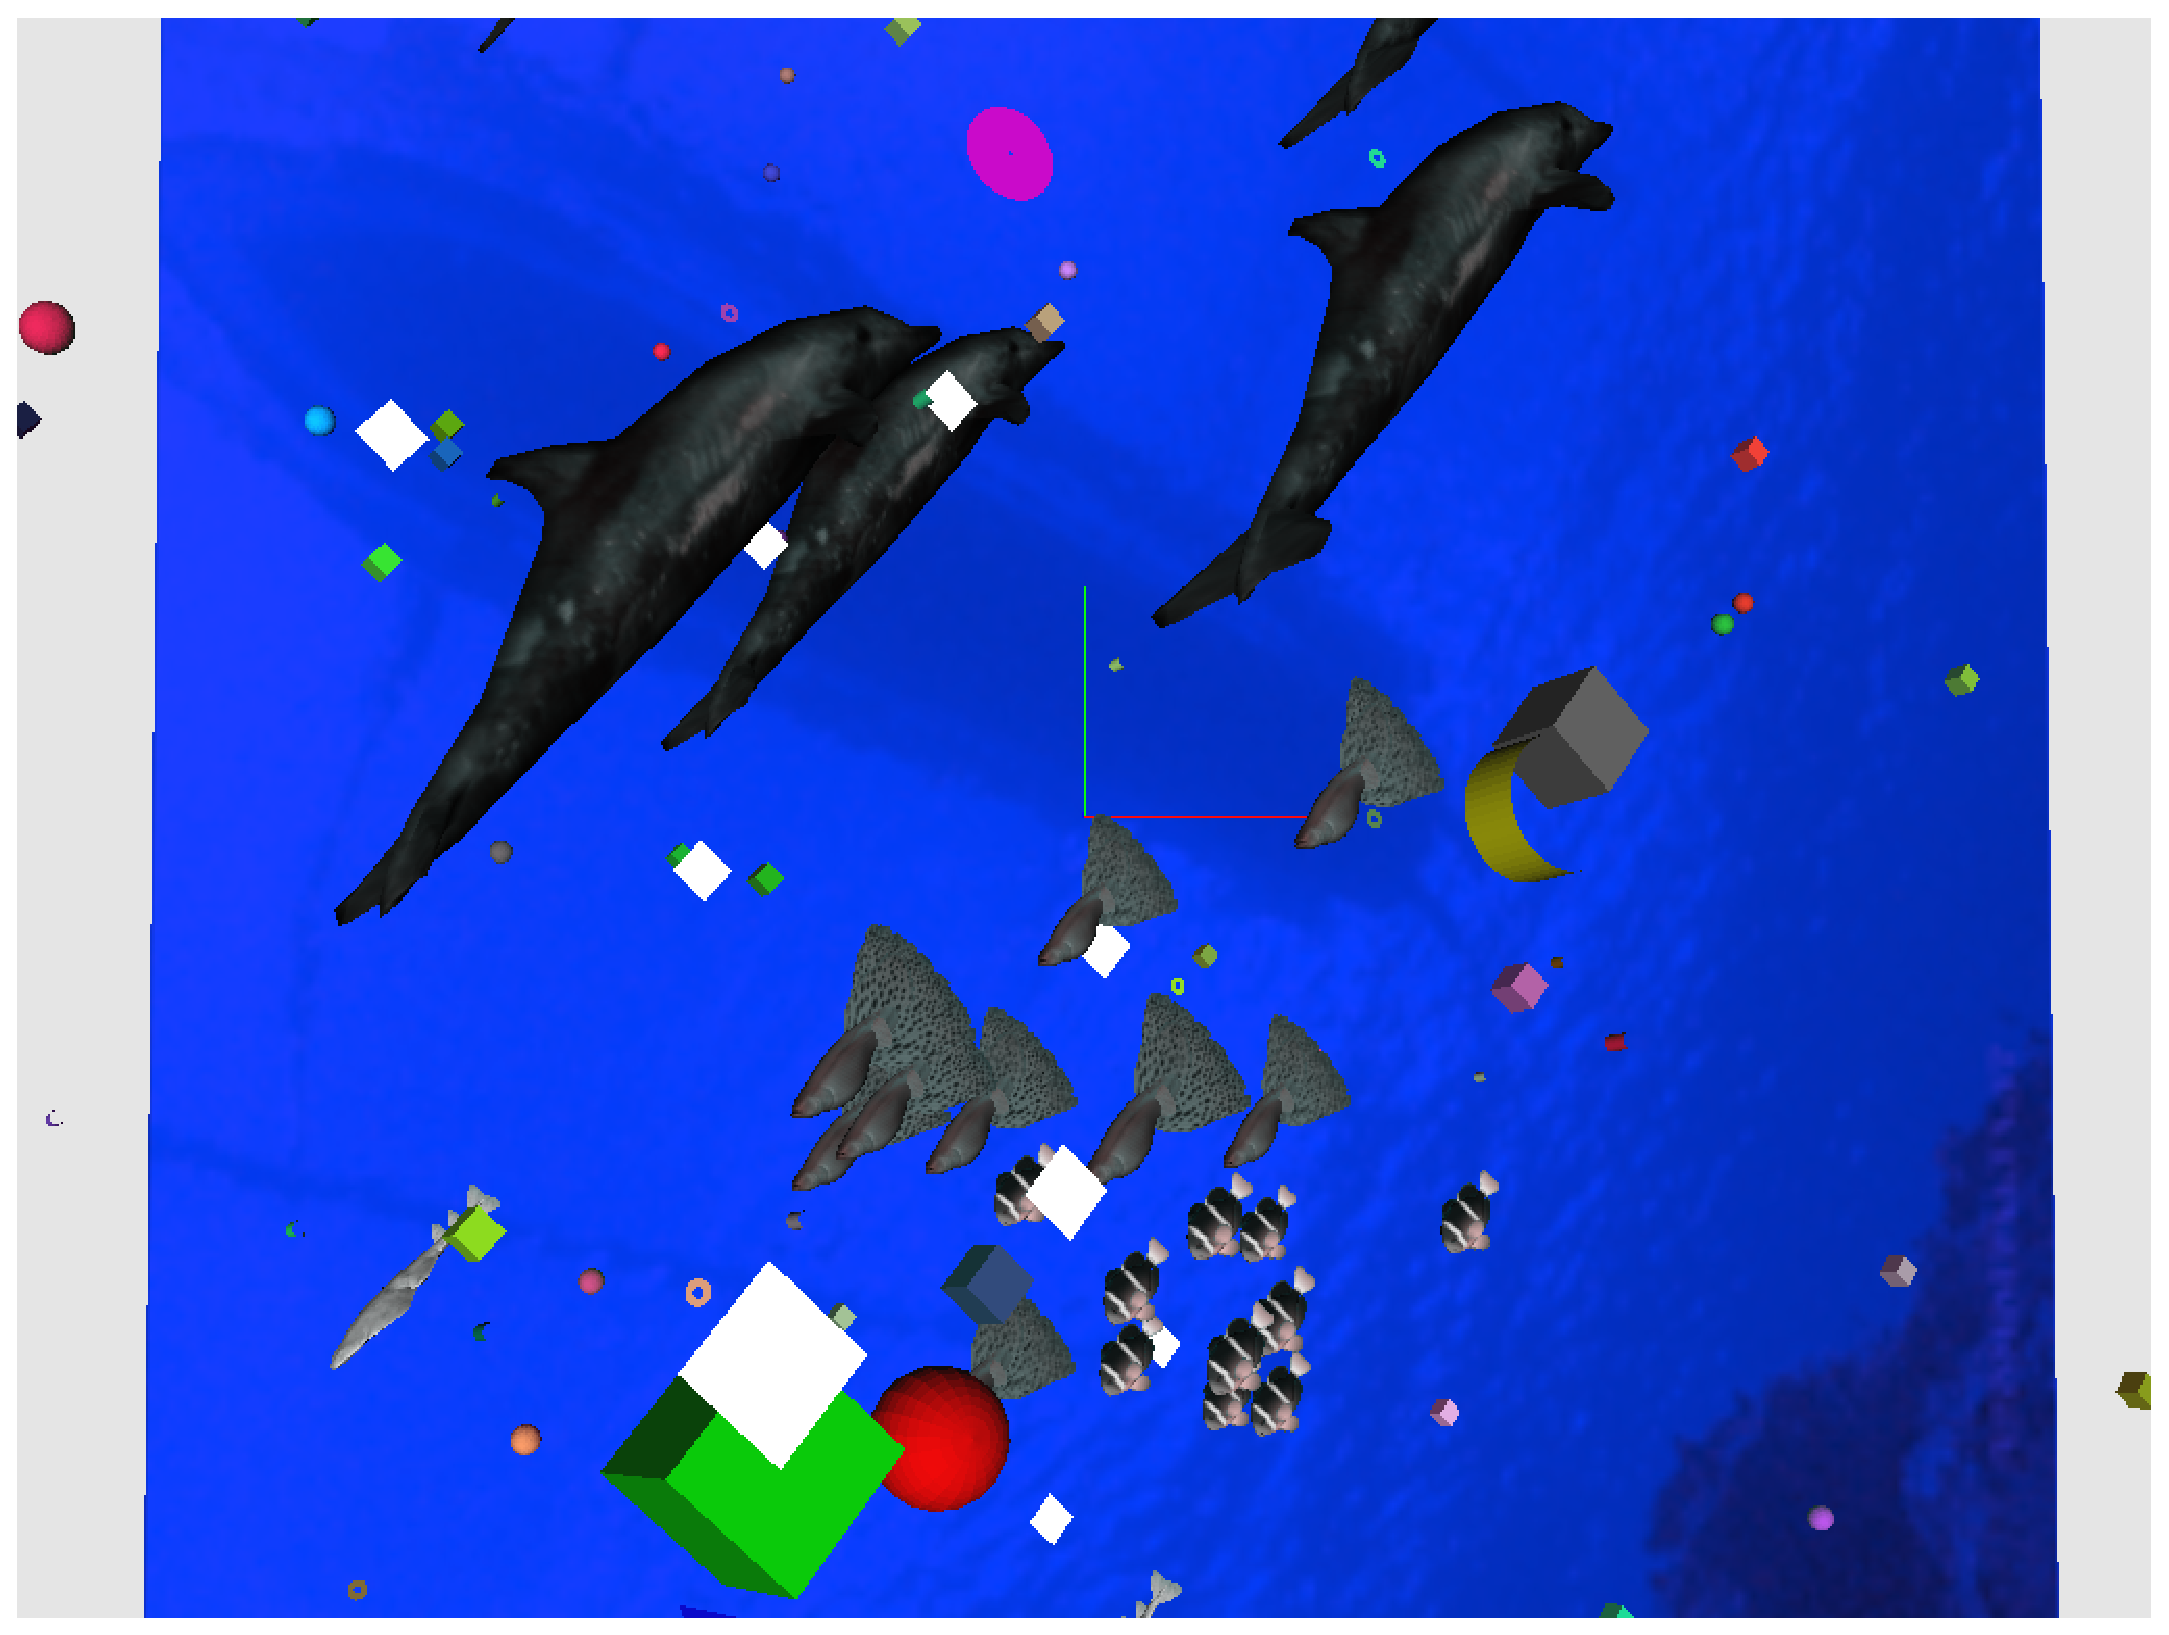
\epsfig{file=scene_example.eps,%
  width=8cm}
\end{center}

\caption{ a) Hierarchical structure in terms of position (big cube, sphere, triangle, cube, and disk). b) 5 schools of fishes: 7 dolpins, 10 Guppy Blue Grasses, 10 Leopard
Sharks, 10 Cuma Domies, and 7 Angel Sharks. The number of triangles of them is
5896, 420, 5198, 6628, and 7144, respectively. Fish structure it self has
hierarchical structure, and the conversion construct scene graph using in-fish and out-fish structures. c) A flat list of Small particles composed of
50 cubes, 30 cylinders, 20 disks, 20 quads, 30 spheres, and 10 triangles.
\label{pic}
}
\end{figure}

The Figure \ref{pic} is a rendering result of scene graph construction. 
This picture shows different transformations from three example domain data structures.


\section{Conclusions and Future Work}
In this paper, we discussed the PLT Scheme implementation of Scene graph. Also presented the way of constructing 
it not from the scratch but from the existing domain-specific structure. We used Mixin class's ability to contain the specification about interfaces for generating tree structures and related nodes. 

We showed how useful the class in PLT scheme is for collecting and manage the necessary data for visualization and user interaction. Especially it maintains the benefit of classes in other language, like C++ or Java. And we can access the data in them using scheme procedures.

For the further research and implementation, it is necessary to support moving object which acutally moves in position and orientation or deformation in itself. It will be interesting how to design the functional API to detect and keep track of current state of time information. 

As the version of OpenGL increases, it is taking more advanced handling of graphics object. Though the current version is working only on version 1.1 and display list is used for faster scene rendering, it is lack of responding quickly when the scene is changed and needs a new display list. The higher version of specification has more flexsible in dealing with various situation on updating the graphics objects and scene structure. So the suppport of the higher feature would be a good direction of implementation.

\appendix

\section{Scheme Structure of Geometric Primitives and Attributes}
This section is to show the structure of graphics primitives. Though they are just a collection of a simpler data structure, they plays an important role as a data type of interface which is necessary for defining and using renderer class. 
{\small
\begin{verbatim}
  ;  position: point3
  ;  normal  : point3
  ;  texture : point2
  (define-struct vertex (position normal texture color))

  (define build-vertex 
    (lambda (position 
             #:n [normal (make-point3 0.0 0.0 1.0)]
             #:t [texture (make-point2 0.5 0.5)]
             #:c [color (make-point4 0.5 0.5 0.5 1.0)])
      (make-vertex position normal texture color)))
                                 
  
  ; point4 point4 point4 number 
  ; (list width:int height:int cvector)
  (define-struct material 
    (ambient diffuse specular shininess texture-object))

  ;; graphics primitive objects
  (define-struct gfx_primitive ())
  (define-struct (line gfx_primitive) 
    (pt_begin pt_end)) ;(point3 point3)
  (define-struct (cube gfx_primitive) 
    (szx szy szz))
  (define-struct (cylinder gfx_primitive) 
    (base_radius top_radius height))
  (define-struct (disk gfx_primitive) 
    (inner_radius outer_radius))
  (define-struct (sphere gfx_primitive) 
    (radius))
  (define-struct (triangle gfx_primitive) 
    (vertex0 vertex1 vertex2))
  (define-struct (quad gfx_primitive) 
    (vertex0 vertex1 vertex2 vertex3))
  (define-struct (surface gfx_primitive) 
    (lst-triangle))

  (define-struct bounding-box (min-posn3 max-posn3))
\end{verbatim}
}

\nocite{Findler06slideshow}

\bibliographystyle{plain}
\bibliography{bib_sglt}



\end{document}
